%-----------------------------------------------------------------
%	PDI CORRELATIONS
%	!TEX root = ./../main.tex
%-----------------------------------------------------------------
\subsection{PDI correlations}\label{sec:pdi-corrs}
\subsubsection{Statistical description}\label{ssec:pdi-corr-stats}
As we mentioned in~\cref{sec:pdi-vs-sst}, we want to find a correlation between the $PDI$ and the duration of the storms, or their wind speeds. Instead of using the whole tropical-cyclones data set as is, we will separate developing from non-developing systems.

Tropical-cyclones that surpass the $\SI{33}{\knot}$ wind speed threshold are called developing systems, whilst the ones that do not do so are called non-developing systems. In terms of hydrodynamics, the major difference between developing and non-developing systems is that the developing have a distinct area of low height or low pressure centred on the system, i.e., they form cyclones~\cite{McBride1979}.

This means that even though all tropical-cyclones behave thermodynamically in the same way throughout their lifetime (the $PDI$ calculation is valid for all their life span), the wind speeds evolve rather differently depending on the development status of the storm. For this reason, we will play on the cautious side and study developing and non-developing systems separately.

\bigskip
\nocite{Domingo2012}
The most common method to find the best fit is the least squares regression. This method
consists in minimising the square of the deviations $y_{i} - \hat{y}_{i}$ where $(x_{i} , y_{i} )$ are the data points ($i = 1, \dots, n$) and $(\hat{x}_{i} , \hat{y}_{i})$ are the expected $(x, y)$ points according to equation
\begin{align}\label{eq:lm-model}
	y = a + b x
\end{align}

\begin{subequations}
More specifically, we have to minimise the sum of the product of the deviation, measured
in absolute values:
\begin{align}
	D^{2} = \sum_{i=1}^{n} \qty(y_{i} - \hat{y}_{i})^{2} = \sum_{i=1}^{n} \qty(y_{i} - a - b x_{i})^{2}
\end{align}
The minimum is reached when
\begin{align}
	\pdv{D^{2}}{a} &= - 2 \sum_{i=1}^{n} (y_{i} - a - b x_{i}) = 0  \label{eq:min-a}\\
	\pdv{D^{2}}{b} &= - 2 \sum_{i=1}^{n} x_{i} (y_{i} - a - b x_{i}) = 0 \label{eq:min-b}
\end{align}
\end{subequations}

From equation \eqref{eq:min-a}, we can show that $a = \bar{y} - b \bar{x}$,
where $\bar{x}$ and $\bar{y}$ are the mean of $x$ and $y$:
\begin{align}
	\bar{x} = \frac{1}{n} \sum_{i=1}^{n} x_{i} \qc \bar{y} = \frac{1}{n} \sum_{i=1}^{n} y_{i}
\end{align}

Replacing $a$ by $\bar{y} - m \bar{x}$ in the equation \eqref{eq:min-b}, we find that the slope is
\begin{align}
	b = \frac{s_{x,y}}{s_{x}^{2}}
\end{align}
where $s_{x}^{2}$ and $s_{x,y}$ are the variance of $x$ and the covariance of $x$ and $y$, respectively:
\begin{subequations}
\begin{align}
	s_{x}^{2} &= \frac{1}{n} \sum_{i=1}^{n} \qty(x_{i} - \bar{x})^{2} \\
	s_{x,y} &= \frac{1}{n} \sum_{i=1}^{n} \qty(x_{i} - \bar{x}) \qty(y_{i} - \bar{y})
\end{align}
\end{subequations}

The equation of our fit is therefore
\begin{align}\label{eq:linear-fit}
	y = \frac{s_{x,y}}{s_{x}^{2}} (x - \bar{x}) + \bar{y}
\end{align}
which passes through the point $(\bar{x}, \bar{y})$.

\sk
The goodness of a fit can be assessed by measuring the correlation coefficient. This
coefficient is given by
\begin{align}
	r = \frac{s_{x,y}}{s_{x} s_{y}} \qc -1 \le r \le 1
\end{align}
where $s_{x} = \sqrt{s_{x}^{2}}$ and $s_{y} = \sqrt{s_{y}^{2}}$ are the standard deviations of $x$ and $y$.

\sk
This linear fit model can be interpreted as a causal relationship between $x$ and $y$. Importantly, causality in this context means the direction of causality runs from $x$ to $y$ and not the other way round.

It's important to notice that the relationships between the $PDI$ and the other variables are of non-linear nature. This naturally means that our regressions need to follow a so-called log--log model:
\begin{align}\label{eq:lm-model-bis}
	\log \eta = a + b \log \epsilon \qc \text{where }
	\log \eta \equiv y \qc
	\log \epsilon \equiv x
	\tag{\ref{eq:lm-model} bis}
\end{align}

We do not know exactly how the $PDI$ and the duration of the storms, or their wind speeds are correlated; we just suspect there is a correlation. For this reason, we will not only compute the $y(x)$ fit for each data set, but also $x(y) = \alpha + \beta y$, which is calculated exactly as above just interchanging the role of $x$ and $y$, and calculate the slope and intercept of the equivalent $x(y)^{-1}$ fit respectively as
\begin{align}
	a' = -\frac{\alpha}{\beta} \qc b' = \frac{1}{\beta}
\end{align}

For the determination of the standard errors $s_{a}$ and $s_{b}$, we will rely on the R \inline{stats} library and the usual error propagation methods.

\bigskip
The hypothesis is that the $\text{SST}$ does not directly affect the maximum wind speed of a tropical-cyclone: storms of equal duration should, in theory, have the same wind speed and $PDI$. Once the cyclone is activated, the wind speed should not depend on the $\text{SST}$.

In essence, our methodology will consist in comparing the low-SST and high-SST fits obtained for each data set. Ideally the equations for both fits should be statistically compatible for developing systems. There is no clear basis to say this about non-developing systems, but we will study them anyhow.

%-----------------------------------------------------------------
\subsubsection{Discussion of the results}\label{ssec:pdi-corr-res}
\subsubsection*{PDI vs storm duration}
In figures \ref{fig:scatter-natl-ds} and \ref{fig:scatter-natl-nds} we can see the $PDI$ vs storm duration regression analyses for the North Atlantic Ocean (developing and non-developing systems, respectively); in figures \ref{fig:scatter-epac-ds} and \ref{fig:scatter-epac-nds} we can see the same analyses for the Northeast Pacific Ocean instead. These figures have been obtained by using the \inline{plot_pdi_scatter_by_status()} function defined in the script~\ref{scr:analysis_base}, in~\cref{app:code}.

A detailed of the statistical coefficients of the regression models we have computed is given in table \ref{tab:pdi-corrs}.

\subsubsection*{PDI vs wind speed}
Regarding the correlation between the $PDI$ and the wind speed, we use the maximum
surface wind speed (in \si{\m\per\s}) sustained over the entire lifetime of the storm as a representative wind speed value of it. Note that we only study developing systems, as the non-developing systems data sets are statistically scarce (the only possible winds speeds are \SIlist[list-units = single]{20;25;30}{\knot}).

In figures \ref{fig:scatter-natl-wind} and \ref{fig:scatter-epac-wind} we can see the $PDI$ vs maximum wind speed regression analyses for the North Atlantic Ocean and the Northeast Pacific Ocean. Note that we have added jitter (a small amount of random variation to the location of each point) to improve the data visualisation, as there are lots of overlapping points. These figures have been obtained by using the \inline{plot_pdi_scatter_wind()} function defined in the script~\ref{scr:analysis_base}, in~\cref{app:code}.

The summary of the statistical coefficients of these regressions can be found in table~\ref{tab:pdi-corrs-wind}.


\subsubsection*{Discussion}
The first thing to notice about the results is that, as it ought to be, the two regression lines, $y(x)$ and $x(y)^{-1}$, for each fitted data set cut at the $(\bar{x}, \bar{y})$ point.

For the comparison of the low-SST and high-SST regression lines, we will use a coverage factor $k = 2 $ to ensure a level of confidence associated with the results of $\SI{95.45}{\percent}$. What we see is that, as we suspected, the SST has no clear influence on the evolution of the tropical-cyclone once it's activated; given a regression model (i.e., $y(x)$ or $x(y)^{-1}$) the two data sets are statistically compatible. This is true for both the $PDI$ vs storm duration and the $PDI$ vs maximum wind speed regressions.

The major difference between the two studied correlations is that the determination coefficient, $r^{2}$, is slightly better for the $PDI$ vs maximum wind speed regression. This should not be too surprising, as there is an explicit physical dependence of the $PDI$ on the sustained surface wind speed, as discussed in \cref{sec:pdi}. If anything, we should be surprised by the fact that the maximum wind speed is such a good representative value of the whole storm.

What we did definitely not expect is that our hypothesis would also be valid for non-developing systems; the correlations in the data are even better than for the developing systems data sets ($r^{2} \sim 0.9$ vs $r^{2} \sim 0.6$), but that could be associated to the low number of storms, resulting in less spread in the data. Having said that, it's a remarkable result.

\bigskip
To finish, we would like to discuss the difference between the $y(x)$ and $x(y)^{-1}$ fits. What one would expect from a perfect correlation is that the $y(x)$ and $x(y)^{-1}$ functions describe the same exact linear equation. By all means, nonetheless, in real-life data the determination coefficient will hardly be $r^{2} \equiv 1$.

The mathematical relationship between $y(x)$ and $x(y)^{-1}$, with respective slopes of $b$ and $b'$, clearly explains this behaviour:
\begin{align}
	b' = \frac{b}{r^{2}}
\end{align}

In our results this is quite unmistakable, the limit $y(x) = x(y)^{-1}$ is truer for higher $r^{2}$ coefficients. This is undoubtedly reflected upon the regression lines themselves: the low-SST $PDI$ vs maximum wind speed regression for the E.~Pac. (figure \ref{fig:scatter-epac-wind}) has the best correlation, whilst both $PDI$ vs storm duration regressions for E.~Pac.'s developing systems (figure \ref{fig:scatter-epac-ds}) have the worst.

%-----------------------------------------------------------------
% \newpage
% \subsubsection{Summary tables}\label{ssec:pdi-corr-sum}
\begin{table}[H]
	\centering
	\begin{tabular}{l l l l c c c }
		\toprule
		\toprule
		Basin & System status & $f(x)$ & SST class & $a$ & $b$ & $r^{2}$ \\
		\midrule
		\multirow{8}{*}{N.~Atl.}
		& \multirow{4}{*}{Developing}
		& \multirow{2}{*}{$y(x)$}
		  & Low  & \num{5.94 \pm 0.18} & \num{1.83 \pm 0.08} & \num{0.67} \\
		& & & High & \num{5.91 \pm 0.17} & \num{1.83 \pm 0.08} & \num{0.62} \\
		\cmidrule(l){3-7}
		& & \multirow{2}{*}{$x(y)^{-1}$}
		  & Low  & \num{3.9 \pm 0.5} & \num{2.74 \pm 0.12} & \num{0.67} \\
		& & & High & \num{3.4 \pm 0.4} & \num{2.97 \pm 0.13} & \num{0.62} \\
		\cmidrule(l){2-7} % \midrule
		& \multirow{4}{*}{Non-developing}
		& \multirow{2}{*}{$y(x)$}
		  & Low  & \num{6.76 \pm 0.07} & \num{1.09 \pm 0.04} & \num{0.88} \\
		& & & High & \num{7.02 \pm 0.08} & \num{0.98 \pm 0.04} & \num{0.89} \\
		\cmidrule(l){3-7}
		& & \multirow{2}{*}{$x(y)^{-1}$}
		  & Low  & \num{6.5 \pm 0.4} & \num{1.24 \pm 0.04} & \num{0.88} \\
		& & & High & \num{6.8 \pm 0.5} & \num{1.09 \pm 0.05} & \num{0.89} \\
% 		\bottomrule
% 	\end{tabular}}
% 	\caption{Summary of the $PDI$ vs duration linear regressions (N.~Atl.)}
% 	\label{tab:pdi-corrs-natl}
% \end{table}

% \begin{table}[H]
% 	\centering
% 	\scalebox{0.95}{
% 	\begin{tabular}{l l l c c c }
		\toprule
		% \toprule
		% System status & $f(x)$ & SST class & $a$ & $b$ & $r^{2}$ \\
		% \midrule
		\multirow{8}{*}{E.~Pac.}
		& \multirow{4}{*}{Developing}
		& \multirow{2}{*}{$y(x)$}
		  & Low  & \num{6.07 \pm 0.18} & \num{1.78 \pm 0.08} & \num{0.59} \\
		& & & High & \num{5.36 \pm 0.18} & \num{2.10 \pm 0.08} & \num{0.60} \\
		\cmidrule(l){3-7}
		& & \multirow{2}{*}{$x(y)^{-1}$}
		  & Low  & \num{3.5 \pm 0.4} & \num{3.00 \pm 0.13} & \num{0.59} \\
		& & & High & \num{2.2 \pm 0.4} & \num{3.53 \pm 0.14} & \num{0.60} \\
		\cmidrule(l){2-7} % \midrule
		& \multirow{4}{*}{Non-developing}
		& \multirow{2}{*}{$y(x)$}
		  & Low  & \num{7.05 \pm 0.11} & \num{0.96 \pm 0.06} & \num{0.87} \\
		& & & High & \num{7.15 \pm 0.09} & \num{0.91 \pm 0.05} & \num{0.85} \\
		\cmidrule(l){3-7}
		& & \multirow{2}{*}{$x(y)^{-1}$}
		  & Low  & \num{6.8 \pm 0.7} & \num{1.09 \pm 0.07} & \num{0.87} \\
		& & & High & \num{6.9 \pm 0.7} & \num{1.07 \pm 0.06} & \num{0.85} \\
		\bottomrule
	\end{tabular}
	\caption{Summary of the $PDI$ vs duration linear regressions}
	\label{tab:pdi-corrs}
\end{table}

\begin{table}[H]
	\centering
	\scalebox{1}{
	\begin{tabular}{l l l c c c }
		\toprule
		\toprule
		Basin & $f(x)$ & SST class & $a$ & $b$ & $r^{2}$ \\
		\midrule
		\multirow{4}{*}{N.~Atl.} &
		\multirow{2}{*}{$y(x)$}
		  & Low  & \num{4.64 \pm 0.14} & \num{3.43 \pm 0.09} & \num{0.85} \\
		& & High & \num{4.90 \pm 0.11} & \num{3.28 \pm 0.07} & \num{0.86} \\
		\cmidrule(l){2-6}
		& \multirow{2}{*}{$x(y)^{-1}$}
		  & Low  & \num{3.7 \pm 0.3}   & \num{4.04 \pm 0.11} & \num{0.85} \\
		& & High & \num{4.10 \pm 0.23} & \num{3.80 \pm 0.08} & \num{0.86} \\
		\midrule
		\multirow{4}{*}{E.~Pac.} &
		\multirow{2}{*}{$y(x)$}
		  & Low  & \num{5.07 \pm 0.09} & \num{3.14 \pm 0.06} & \num{0.87} \\
		& & High & \num{4.94 \pm 0.07} & \num{3.23 \pm 0.04} & \num{0.93} \\
		\cmidrule(l){2-6}
		& \multirow{2}{*}{$x(y)^{-1}$}
		  & Low  & \num{4.37 \pm 0.21} & \num{3.60 \pm 0.07} & \num{0.87} \\
		& & High & \num{4.54 \pm 0.15} & \num{3.48 \pm 0.05} & \num{0.93} \\
		\bottomrule
	\end{tabular}}
	\caption{Summary of the $PDI$ vs maximum wind speed linear regressions for developing systems}
	\label{tab:pdi-corrs-wind}
\end{table}

%-----------------------------------------------------------------
\newpage
\subsubsection{PDI vs storm duration scatterplots}\label{ssec:pdi-corr-duration}
\begin{figure}[H]
	\centering
	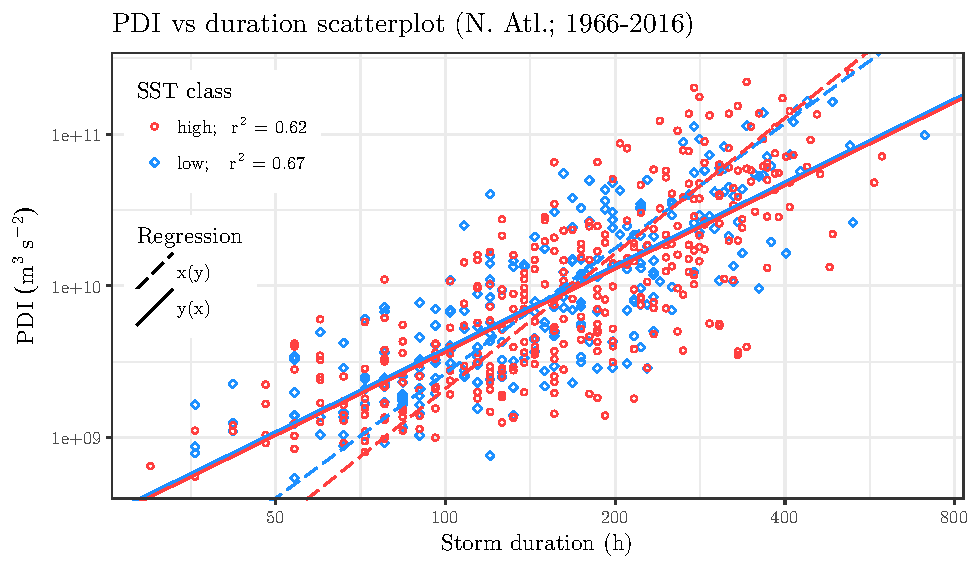
\includegraphics[width=\textwidth]{images/scatter-natl-ds}
	\caption{$PDI$ vs duration analysis for developing systems (N.~Atl.)}
	\label{fig:scatter-natl-ds}
\end{figure}

\begin{figure}[H]
	\centering
	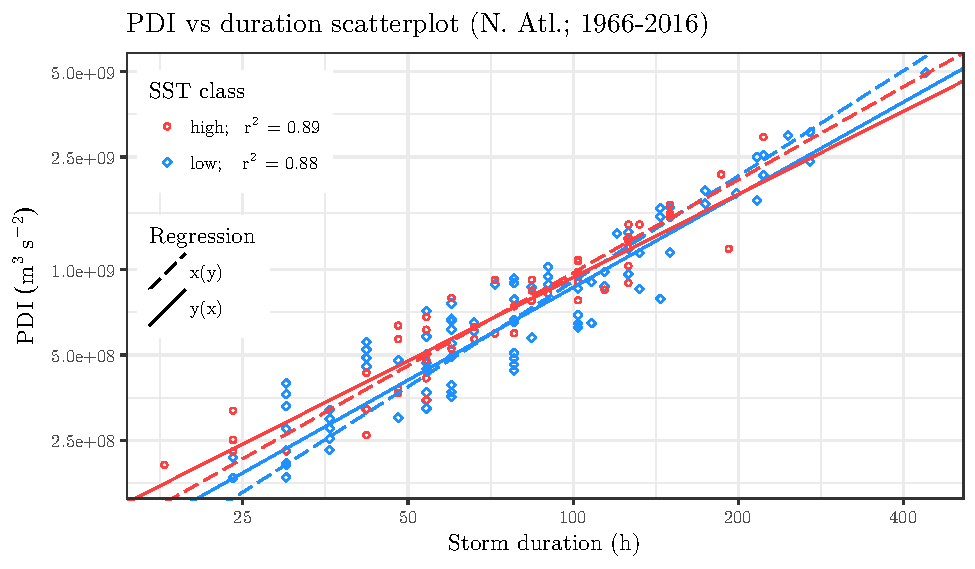
\includegraphics[width=\textwidth]{images/scatter-natl-nds}
	\caption{$PDI$ vs duration analysis for non-developing systems (N.~Atl.)}
	\label{fig:scatter-natl-nds}
\end{figure}

\begin{figure}[H]
	\centering
	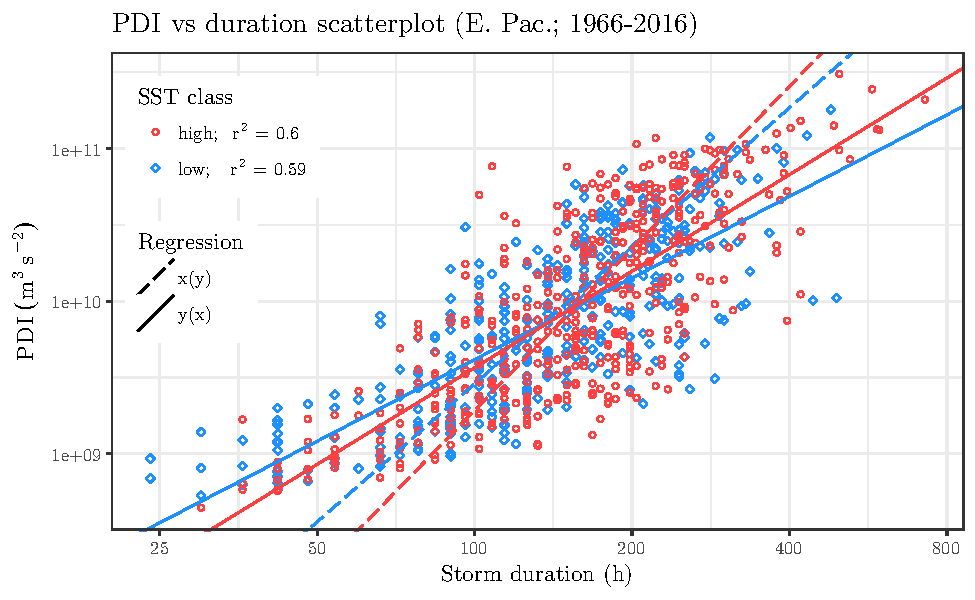
\includegraphics[width=\textwidth]{images/scatter-epac-ds}
	\caption{$PDI$ vs duration analysis for developing systems (E.~Pac.)}
	\label{fig:scatter-epac-ds}
\end{figure}

\begin{figure}[H]
	\centering
	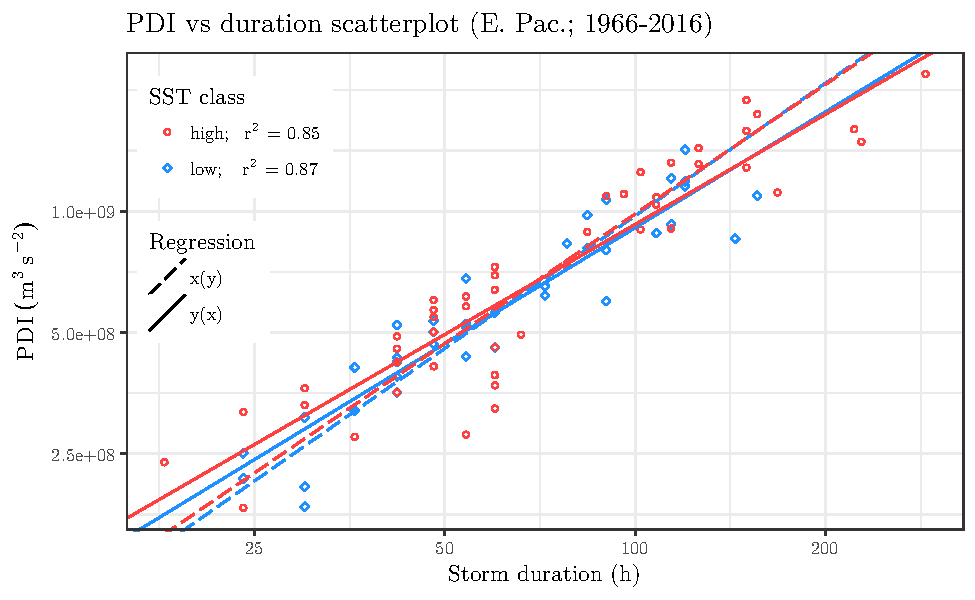
\includegraphics[width=\textwidth]{images/scatter-epac-nds}
	\caption{$PDI$ vs duration analysis for non-developing systems (E.~Pac.)}
	\label{fig:scatter-epac-nds}
\end{figure}

%-----------------------------------------------------------------
\newpage
\subsubsection{PDI vs wind speed scatterplots}\label{ssec:pdi-corr-speed}
\begin{figure}[H]
	\centering
	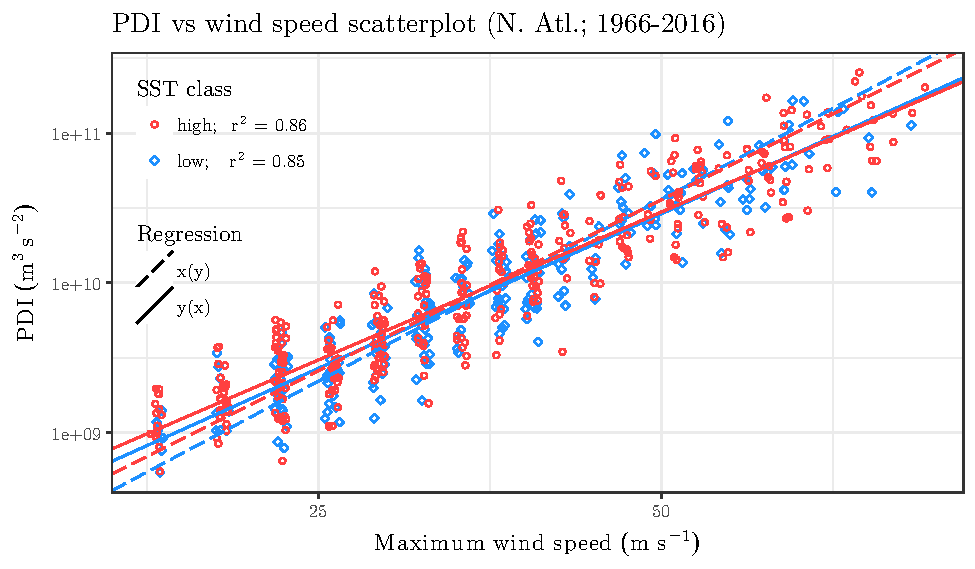
\includegraphics[width=\textwidth]{images/scatter-natl-wind}
	\caption{$PDI$ vs maximum wind speed analysis for developing systems (N.~Atl.)}
	\label{fig:scatter-natl-wind}
\end{figure}

\begin{figure}[H]
	\centering
	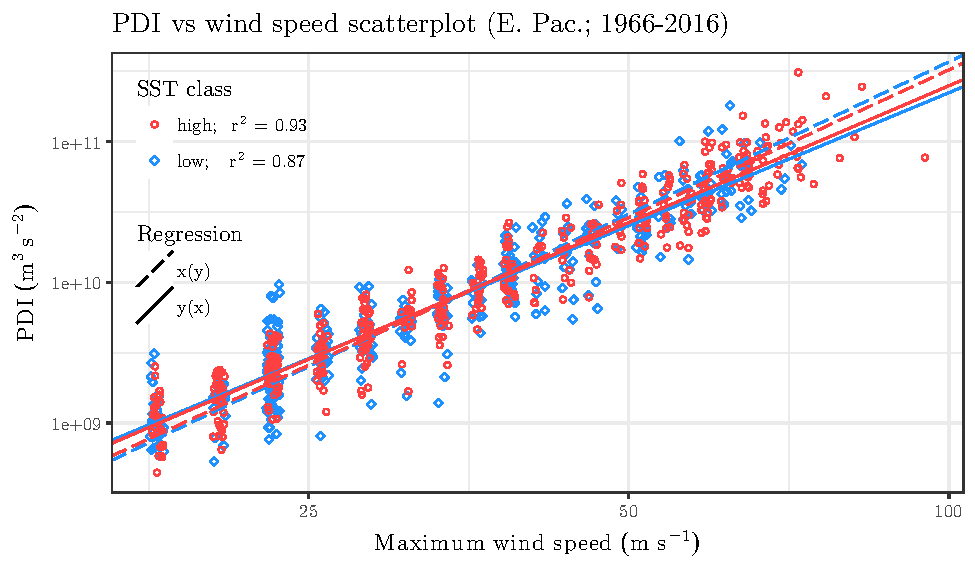
\includegraphics[width=\textwidth]{images/scatter-epac-wind}
	\caption{$PDI$ vs maximum wind speed analysis for developing systems (E.~Pac.)}
	\label{fig:scatter-epac-wind}
\end{figure}

% \begin{table}[H]
% 	\centering
% 	\begin{tabular}{l l c c c }
% 		\toprule
% 		\toprule
% 		$f(x)$ & SST class & $a$ & $b$ & $r^{2}$ \\
% 		\midrule
% 		\multirow{2}{*}{$y(x)$} &
% 		  Low  & \num{4.64 \pm 0.14} & \num{3.43 \pm 0.09} & \num{0.85} \\
% 		& High & \num{4.90 \pm 0.11} & \num{3.28 \pm 0.07} & \num{0.86} \\
% 		\cmidrule(l){2-5}
% 		\multirow{2}{*}{$x(y)^{-1}$}
% 		& Low  & \num{3.7 \pm 0.3}   & \num{4.04 \pm 0.11} & \num{0.85} \\
% 		& High & \num{4.10 \pm 0.23} & \num{3.80 \pm 0.08} & \num{0.86} \\
% 		\bottomrule
% 	\end{tabular}
% 	\caption{Summary of the $PDI$ vs maximum wind speed linear regressions (N.~Atl.)}
% 	\label{tab:pdi-corrs-natl-wind}
% \end{table}

% \begin{table}[H]
% 	\centering
% 	\begin{tabular}{c l c c c }
% 		\toprule
% 		\toprule
% 		$f(x)$ & SST class & $a$ & $b$ & $r^{2}$ \\
% 		\midrule
% 		\multirow{2}{*}{$y(x)$} &
% 		  Low  & \num{5.07 \pm 0.09} & \num{3.14 \pm 0.06} & \num{0.87} \\
% 		& High & \num{4.94 \pm 0.07} & \num{3.23 \pm 0.04} & \num{0.93} \\
% 		\cmidrule(l){2-5}
% 		\multirow{2}{*}{$x(y)^{-1}$}
% 		& Low  & \num{4.37 \pm 0.21} & \num{3.60 \pm 0.07} & \num{0.87} \\
% 		& High & \num{4.54 \pm 0.15} & \num{3.48 \pm 0.05} & \num{0.93} \\
% 		\bottomrule
% 	\end{tabular}
% 	\caption{Summary of the $PDI$ vs maximum wind speed linear regressions (E.~Pac.)}
% 	\label{tab:pdi-corrs-epac-wind}
% \end{table}

